% Graphic for TeX using PGF
% Title: Z:\people\stephen\GlobalDocs\Projects\IPMAS\Architecture\Metric Taxonomy.dia
% Creator: Dia v0.97.2
% CreationDate: Thu Nov 01 11:07:49 2012
% For: stephen
% \usepackage{tikz}
% The following commands are not supported in PSTricks at present
% We define them conditionally, so when they are implemented,
% this pgf file will use them.
\ifx\du\undefined
  \newlength{\du}
\fi
\setlength{\du}{15\unitlength}
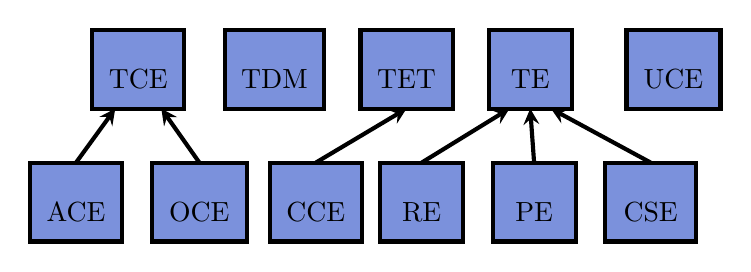
\begin{tikzpicture}
\pgftransformxscale{1.000000}
\pgftransformyscale{-1.000000}
\definecolor{dialinecolor}{rgb}{0.000000, 0.000000, 0.000000}
\pgfsetstrokecolor{dialinecolor}
\definecolor{dialinecolor}{rgb}{1.000000, 1.000000, 1.000000}
\pgfsetfillcolor{dialinecolor}
\definecolor{dialinecolor}{rgb}{0.480705, 0.569238, 0.861845}
\pgfsetfillcolor{dialinecolor}
\fill (1.257500\du,13.800000\du)--(1.257500\du,15.700000\du)--(3.487500\du,15.700000\du)--(3.487500\du,13.800000\du)--cycle;
\pgfsetlinewidth{0.100000\du}
\pgfsetdash{}{0pt}
\pgfsetdash{}{0pt}
\pgfsetmiterjoin
\definecolor{dialinecolor}{rgb}{0.000000, 0.000000, 0.000000}
\pgfsetstrokecolor{dialinecolor}
\draw (1.257500\du,13.800000\du)--(1.257500\du,15.700000\du)--(3.487500\du,15.700000\du)--(3.487500\du,13.800000\du)--cycle;
% setfont left to latex
\definecolor{dialinecolor}{rgb}{0.000000, 0.000000, 0.000000}
\pgfsetstrokecolor{dialinecolor}
\node at (2.372500\du,14.990000\du){ACE};
\definecolor{dialinecolor}{rgb}{0.480705, 0.569238, 0.861845}
\pgfsetfillcolor{dialinecolor}
\fill (4.194844\du,13.800000\du)--(4.194844\du,15.700000\du)--(6.492344\du,15.700000\du)--(6.492344\du,13.800000\du)--cycle;
\pgfsetlinewidth{0.100000\du}
\pgfsetdash{}{0pt}
\pgfsetdash{}{0pt}
\pgfsetmiterjoin
\definecolor{dialinecolor}{rgb}{0.000000, 0.000000, 0.000000}
\pgfsetstrokecolor{dialinecolor}
\draw (4.194844\du,13.800000\du)--(4.194844\du,15.700000\du)--(6.492344\du,15.700000\du)--(6.492344\du,13.800000\du)--cycle;
% setfont left to latex
\definecolor{dialinecolor}{rgb}{0.000000, 0.000000, 0.000000}
\pgfsetstrokecolor{dialinecolor}
\node at (5.343594\du,14.990000\du){OCE};
\definecolor{dialinecolor}{rgb}{0.480705, 0.569238, 0.861845}
\pgfsetfillcolor{dialinecolor}
\fill (2.762500\du,10.600000\du)--(2.762500\du,12.500000\du)--(4.982500\du,12.500000\du)--(4.982500\du,10.600000\du)--cycle;
\pgfsetlinewidth{0.100000\du}
\pgfsetdash{}{0pt}
\pgfsetdash{}{0pt}
\pgfsetmiterjoin
\definecolor{dialinecolor}{rgb}{0.000000, 0.000000, 0.000000}
\pgfsetstrokecolor{dialinecolor}
\draw (2.762500\du,10.600000\du)--(2.762500\du,12.500000\du)--(4.982500\du,12.500000\du)--(4.982500\du,10.600000\du)--cycle;
% setfont left to latex
\definecolor{dialinecolor}{rgb}{0.000000, 0.000000, 0.000000}
\pgfsetstrokecolor{dialinecolor}
\node at (3.872500\du,11.790000\du){TCE};
\definecolor{dialinecolor}{rgb}{0.480705, 0.569238, 0.861845}
\pgfsetfillcolor{dialinecolor}
\fill (5.952031\du,10.600000\du)--(5.952031\du,12.500000\du)--(8.354531\du,12.500000\du)--(8.354531\du,10.600000\du)--cycle;
\pgfsetlinewidth{0.100000\du}
\pgfsetdash{}{0pt}
\pgfsetdash{}{0pt}
\pgfsetmiterjoin
\definecolor{dialinecolor}{rgb}{0.000000, 0.000000, 0.000000}
\pgfsetstrokecolor{dialinecolor}
\draw (5.952031\du,10.600000\du)--(5.952031\du,12.500000\du)--(8.354531\du,12.500000\du)--(8.354531\du,10.600000\du)--cycle;
% setfont left to latex
\definecolor{dialinecolor}{rgb}{0.000000, 0.000000, 0.000000}
\pgfsetstrokecolor{dialinecolor}
\node at (7.153281\du,11.790000\du){TDM};
\definecolor{dialinecolor}{rgb}{0.480705, 0.569238, 0.861845}
\pgfsetfillcolor{dialinecolor}
\fill (9.224062\du,10.600000\du)--(9.224062\du,12.500000\du)--(11.444062\du,12.500000\du)--(11.444062\du,10.600000\du)--cycle;
\pgfsetlinewidth{0.100000\du}
\pgfsetdash{}{0pt}
\pgfsetdash{}{0pt}
\pgfsetmiterjoin
\definecolor{dialinecolor}{rgb}{0.000000, 0.000000, 0.000000}
\pgfsetstrokecolor{dialinecolor}
\draw (9.224062\du,10.600000\du)--(9.224062\du,12.500000\du)--(11.444062\du,12.500000\du)--(11.444062\du,10.600000\du)--cycle;
% setfont left to latex
\definecolor{dialinecolor}{rgb}{0.000000, 0.000000, 0.000000}
\pgfsetstrokecolor{dialinecolor}
\node at (10.334062\du,11.790000\du){TET};
\definecolor{dialinecolor}{rgb}{0.480705, 0.569238, 0.861845}
\pgfsetfillcolor{dialinecolor}
\fill (9.699687\du,13.800000\du)--(9.699687\du,15.700000\du)--(11.699687\du,15.700000\du)--(11.699687\du,13.800000\du)--cycle;
\pgfsetlinewidth{0.100000\du}
\pgfsetdash{}{0pt}
\pgfsetdash{}{0pt}
\pgfsetmiterjoin
\definecolor{dialinecolor}{rgb}{0.000000, 0.000000, 0.000000}
\pgfsetstrokecolor{dialinecolor}
\draw (9.699687\du,13.800000\du)--(9.699687\du,15.700000\du)--(11.699687\du,15.700000\du)--(11.699687\du,13.800000\du)--cycle;
% setfont left to latex
\definecolor{dialinecolor}{rgb}{0.000000, 0.000000, 0.000000}
\pgfsetstrokecolor{dialinecolor}
\node at (10.699687\du,14.990000\du){RE};
\definecolor{dialinecolor}{rgb}{0.480705, 0.569238, 0.861845}
\pgfsetfillcolor{dialinecolor}
\fill (12.407031\du,13.800000\du)--(12.407031\du,15.700000\du)--(14.407031\du,15.700000\du)--(14.407031\du,13.800000\du)--cycle;
\pgfsetlinewidth{0.100000\du}
\pgfsetdash{}{0pt}
\pgfsetdash{}{0pt}
\pgfsetmiterjoin
\definecolor{dialinecolor}{rgb}{0.000000, 0.000000, 0.000000}
\pgfsetstrokecolor{dialinecolor}
\draw (12.407031\du,13.800000\du)--(12.407031\du,15.700000\du)--(14.407031\du,15.700000\du)--(14.407031\du,13.800000\du)--cycle;
% setfont left to latex
\definecolor{dialinecolor}{rgb}{0.000000, 0.000000, 0.000000}
\pgfsetstrokecolor{dialinecolor}
\node at (13.407031\du,14.990000\du){PE};
\definecolor{dialinecolor}{rgb}{0.480705, 0.569238, 0.861845}
\pgfsetfillcolor{dialinecolor}
\fill (15.114375\du,13.800000\du)--(15.114375\du,15.700000\du)--(17.316875\du,15.700000\du)--(17.316875\du,13.800000\du)--cycle;
\pgfsetlinewidth{0.100000\du}
\pgfsetdash{}{0pt}
\pgfsetdash{}{0pt}
\pgfsetmiterjoin
\definecolor{dialinecolor}{rgb}{0.000000, 0.000000, 0.000000}
\pgfsetstrokecolor{dialinecolor}
\draw (15.114375\du,13.800000\du)--(15.114375\du,15.700000\du)--(17.316875\du,15.700000\du)--(17.316875\du,13.800000\du)--cycle;
% setfont left to latex
\definecolor{dialinecolor}{rgb}{0.000000, 0.000000, 0.000000}
\pgfsetstrokecolor{dialinecolor}
\node at (16.215625\du,14.990000\du){CSE};
\definecolor{dialinecolor}{rgb}{0.480705, 0.569238, 0.861845}
\pgfsetfillcolor{dialinecolor}
\fill (12.313594\du,10.600000\du)--(12.313594\du,12.500000\du)--(14.313594\du,12.500000\du)--(14.313594\du,10.600000\du)--cycle;
\pgfsetlinewidth{0.100000\du}
\pgfsetdash{}{0pt}
\pgfsetdash{}{0pt}
\pgfsetmiterjoin
\definecolor{dialinecolor}{rgb}{0.000000, 0.000000, 0.000000}
\pgfsetstrokecolor{dialinecolor}
\draw (12.313594\du,10.600000\du)--(12.313594\du,12.500000\du)--(14.313594\du,12.500000\du)--(14.313594\du,10.600000\du)--cycle;
% setfont left to latex
\definecolor{dialinecolor}{rgb}{0.000000, 0.000000, 0.000000}
\pgfsetstrokecolor{dialinecolor}
\node at (13.313594\du,11.790000\du){TE};
\definecolor{dialinecolor}{rgb}{0.480705, 0.569238, 0.861845}
\pgfsetfillcolor{dialinecolor}
\fill (15.633125\du,10.600000\du)--(15.633125\du,12.500000\du)--(17.898125\du,12.500000\du)--(17.898125\du,10.600000\du)--cycle;
\pgfsetlinewidth{0.100000\du}
\pgfsetdash{}{0pt}
\pgfsetdash{}{0pt}
\pgfsetmiterjoin
\definecolor{dialinecolor}{rgb}{0.000000, 0.000000, 0.000000}
\pgfsetstrokecolor{dialinecolor}
\draw (15.633125\du,10.600000\du)--(15.633125\du,12.500000\du)--(17.898125\du,12.500000\du)--(17.898125\du,10.600000\du)--cycle;
% setfont left to latex
\definecolor{dialinecolor}{rgb}{0.000000, 0.000000, 0.000000}
\pgfsetstrokecolor{dialinecolor}
\node at (16.765625\du,11.790000\du){UCE};
\pgfsetlinewidth{0.100000\du}
\pgfsetdash{}{0pt}
\pgfsetdash{}{0pt}
\pgfsetbuttcap
{
\definecolor{dialinecolor}{rgb}{0.000000, 0.000000, 0.000000}
\pgfsetfillcolor{dialinecolor}
% was here!!!
\pgfsetarrowsend{stealth}
\definecolor{dialinecolor}{rgb}{0.000000, 0.000000, 0.000000}
\pgfsetstrokecolor{dialinecolor}
\draw (2.372500\du,13.800000\du)--(3.317500\du,12.500000\du);
}
\pgfsetlinewidth{0.100000\du}
\pgfsetdash{}{0pt}
\pgfsetdash{}{0pt}
\pgfsetbuttcap
{
\definecolor{dialinecolor}{rgb}{0.000000, 0.000000, 0.000000}
\pgfsetfillcolor{dialinecolor}
% was here!!!
\pgfsetarrowsend{stealth}
\definecolor{dialinecolor}{rgb}{0.000000, 0.000000, 0.000000}
\pgfsetstrokecolor{dialinecolor}
\draw (5.343594\du,13.800000\du)--(4.427500\du,12.500000\du);
}
\pgfsetlinewidth{0.100000\du}
\pgfsetdash{}{0pt}
\pgfsetdash{}{0pt}
\pgfsetbuttcap
{
\definecolor{dialinecolor}{rgb}{0.000000, 0.000000, 0.000000}
\pgfsetfillcolor{dialinecolor}
% was here!!!
\pgfsetarrowsend{stealth}
\definecolor{dialinecolor}{rgb}{0.000000, 0.000000, 0.000000}
\pgfsetstrokecolor{dialinecolor}
\draw (10.699687\du,13.800000\du)--(12.813594\du,12.500000\du);
}
\pgfsetlinewidth{0.100000\du}
\pgfsetdash{}{0pt}
\pgfsetdash{}{0pt}
\pgfsetbuttcap
{
\definecolor{dialinecolor}{rgb}{0.000000, 0.000000, 0.000000}
\pgfsetfillcolor{dialinecolor}
% was here!!!
\pgfsetarrowsend{stealth}
\definecolor{dialinecolor}{rgb}{0.000000, 0.000000, 0.000000}
\pgfsetstrokecolor{dialinecolor}
\draw (13.407031\du,13.800000\du)--(13.313594\du,12.500000\du);
}
\pgfsetlinewidth{0.100000\du}
\pgfsetdash{}{0pt}
\pgfsetdash{}{0pt}
\pgfsetbuttcap
{
\definecolor{dialinecolor}{rgb}{0.000000, 0.000000, 0.000000}
\pgfsetfillcolor{dialinecolor}
% was here!!!
\pgfsetarrowsend{stealth}
\definecolor{dialinecolor}{rgb}{0.000000, 0.000000, 0.000000}
\pgfsetstrokecolor{dialinecolor}
\draw (16.215625\du,13.800000\du)--(13.813594\du,12.500000\du);
}
\definecolor{dialinecolor}{rgb}{0.480705, 0.569238, 0.861845}
\pgfsetfillcolor{dialinecolor}
\fill (7.035000\du,13.800000\du)--(7.035000\du,15.700000\du)--(9.265000\du,15.700000\du)--(9.265000\du,13.800000\du)--cycle;
\pgfsetlinewidth{0.100000\du}
\pgfsetdash{}{0pt}
\pgfsetdash{}{0pt}
\pgfsetmiterjoin
\definecolor{dialinecolor}{rgb}{0.000000, 0.000000, 0.000000}
\pgfsetstrokecolor{dialinecolor}
\draw (7.035000\du,13.800000\du)--(7.035000\du,15.700000\du)--(9.265000\du,15.700000\du)--(9.265000\du,13.800000\du)--cycle;
% setfont left to latex
\definecolor{dialinecolor}{rgb}{0.000000, 0.000000, 0.000000}
\pgfsetstrokecolor{dialinecolor}
\node at (8.150000\du,14.990000\du){CCE};
\pgfsetlinewidth{0.100000\du}
\pgfsetdash{}{0pt}
\pgfsetdash{}{0pt}
\pgfsetbuttcap
{
\definecolor{dialinecolor}{rgb}{0.000000, 0.000000, 0.000000}
\pgfsetfillcolor{dialinecolor}
% was here!!!
\pgfsetarrowsend{stealth}
\definecolor{dialinecolor}{rgb}{0.000000, 0.000000, 0.000000}
\pgfsetstrokecolor{dialinecolor}
\draw (8.150000\du,13.800000\du)--(10.334062\du,12.500000\du);
}
\end{tikzpicture}
